% !TeX encoding = UTF-8
% !TeX spellcheck = hu_HU

\chapter{Monitoring}
\Aref{sect:monitoring}.~alfejezetben ismertetett előnyei miatt a tesztkörnyezetben is egy monitoring rendszer kialakítása mellett döntöttem. Választásom a Prometheus monitorozó rendszerre esett, mely a Grafana vizualizációs eszközzel társítva jó betekintést enged az üzemeltetett rendszerek állapotába. A választásomat az indokolta, hogy ez a párosítás manapság nagyon elterjedt, széles körben használt és jól kibővíthető további adatok monitorozásával, továbbá számos segédanyag áll hozzá rendelkezésre mind a hivatalos oldalon, mind pedig a közösség által karbantartott ismertetők formájában.

\section{Áttekintés}
A továbbiakban tárgyaltak könnyebb megértése végett hasznos megismerni a Prometheus és a kapcsolódó komponensek működését. A Prometheus működési elve egyszerű és hatékony: a figyelt kliensekre úgynevezett \textit{exporter}eket telepítünk, melyeket a Prometheus szerver pull modellt alkalmazva adott időközönként lekérdez. Az exporterek olyan programok, melyek alkalmasak bizonyos statisztikák (pl.~erőforráskihasználtság mértéke, adatbázis-lekérdezések gyakorisága) kiolvasására, és ezeket a monitorozott rendszer egy adott portján HTTP-protokollon keresztül közzétenni. Az exporterek önmagukban nem gyűjtenek adatokat, csak adott időközönként frissítik őket, az adatgyűjtést a Prometheus szerver végzi. Figyelt végpontokból rendszerenként több is lehet, mindegyikhez külön-külön port kapcsolódik.

A monitorozás szerves része a riasztások küldése, hiszen a monitoring rendszer folyamatos figyelése nélkül is jó, ha értesülünk a fennálló problémákról, hogy még időben be tudjunk avatkozni. A Prometheus az riasztások kezeléséhez az Alertmanager komponenst kínálja. Ezt részletesen konfigurálhatjuk az igényeinknek megfelelően, hogy milyen típusú problémáról, milyen platformon keresztül és kik kapjanak értesítést. Ez azért is kedvező, mert például egy éles környezet esetében egy alkalmazás összeomlásakor feltehetőleg másnak kell eljárnia, mint amikor hálózati fennakadást (pl.~\acrshort{dns}-probléma) tapasztalunk.

Az összegyűjtött adatokat a Grafana segítségével tehetjük átláthatóbbá, valamint ez teszi könnyebbé a metrikák elemzését is. Adatvizualizációra specializálódott szoftver lévén a Grafana rengeteg opcióval rendelkezik az adatok megjelenítését illetően, így a \acrshort{cpu}-adatok vonalgrafikonon való megjelenítésétől kezdve a szerverünk elérhetőségét jelző igen-nem panelt is választhatunk.
Grafanában a megjelenített adatokat -- melyekhez egy-egy panel tartozik -- úgynevezett \textit{dashboard}okba szervezhetjük. A dashboardok általában összetartozó adatokat tartalmaznak, azaz jó gyakorlat a hardveres erőforrások metrikáit külön dashboardba szervezni például a webszerverhez tartozó mérőszámoktól. % TODO: összesítés dashboard, amin a monitorozott hosztok adatai egy helyen láthatóak?
A Grafana támogatja a Prometheus saját lekérdezőnyelvével, a PromQL-lel való adatszűrést, mely lehetővé teszi a Prometheus szerverrel való egyszerű interakciót.
\Aref{fig:prometheus-architecture}.~ábra egy általános Prometheus-alapú, Grafana adatvizualizációt használó monitoring-architektúrát mutat be.

% tikz ábra beszúrása
\vspace{0.25cm}
\begin{figure}[ht]
	\centering
	\begin{tikzpicture}[node distance=5cm]
	% Define styles
	\tikzstyle{rect} = [rectangle, draw, minimum width=4.2cm, minimum height=2cm, text centered, font=\fontsize{12}{12}\selectfont]
	\tikzstyle{arrow} = [->,>=stealth]
	
	% Nodes
	\node (monitored-host) [rect, rounded corners, align=center, double copy shadow, fill=white] {Monitorozott\\szolgáltatások\\(exporterek)};
	\node (prometheus) [rect, rounded corners, below right of = monitored-host, yshift=-0.5cm] {Prometheus szerver};
	\node (alertmanager) [rect, rounded corners, above right of = prometheus, yshift=0.5cm, align=center] {Prometheus\\Alertmanager};
	\node (grafana) [rect, rounded corners, below of = prometheus, yshift=1cm] {Grafana};
	
	% Arrows
	\draw [arrow] (prometheus) to node[midway, fill=white, inner sep=2pt, align=center] {Metrikák lekérdezése\\(HTTP-kérések)} (monitored-host);
	\draw [arrow] (prometheus) to node[midway, fill=white, inner sep=2pt] {Riasztások} (alertmanager);
	\draw [arrow] (grafana) to node[midway, fill=white, inner sep=2pt] {Adatok lekérdezése} (prometheus);
\end{tikzpicture}

	\caption{A Prometheus monitoring rendszer felépítése~\cite{PrometheusIntro}.}
	\label{fig:prometheus-architecture}
\end{figure}

A Prometheus exporterek egy speciális formátumban teszik közzé az általuk kinyert adatokat. A legegyszerűbb esetben ezek szóközzel elválasztott kulcs-érték párok. Ilyen adatpárra mutat példát \aref{lst:prometheus-data-format}.~kódrészlet első~sora. A mérőszám elnevezése után kapcsos zárójelekbe szűrőket~(filter) helyezhetünk, ahogy az \aref{lst:prometheus-data-format}.~kódrészlet második~sorában is látható. Lekérdezés esetén az adatokat ugyanezzel a szintaktikával szűrhetjük.
% TODO: lekérdezésre példa

\begin{lstlisting}[caption=Prometheus exporterek által közzétett adatok.,label=lst:prometheus-data-format, numbers=left]
	node_load1 0.35
	node_hwmon_temp_celsius{chip="platform_coretemp_1",sensor="temp2"} 28
\end{lstlisting}

\section{Telepítés, konfiguráció}
A környezet beüzemelését nagyban segítette, hogy a Prometheus monitoring rendszert az Uyuni külön Salt~Formulákon keresztül támogatja. Így lehetőség van az infrastruktúramenedzsment rendszerbe bevont klienseken manuális csomagtelepítés nélkül egy kezdetleges monitoring környezetet kialakítani. Ez a gyakorlatban azt jelentette, hogy az Uyuni a beállított Formulák alapján a kliensekre telepítette az alapvető rendszerinformációkat lekérdező \textit{Node exportert}, míg a monitoring szerveren egy alapbeállításokkal rendelkező Prometheus szervert és a hozzá kapcsolódó Grafana szervert telepítette.


\begin{figure}[ht]
	\centering
	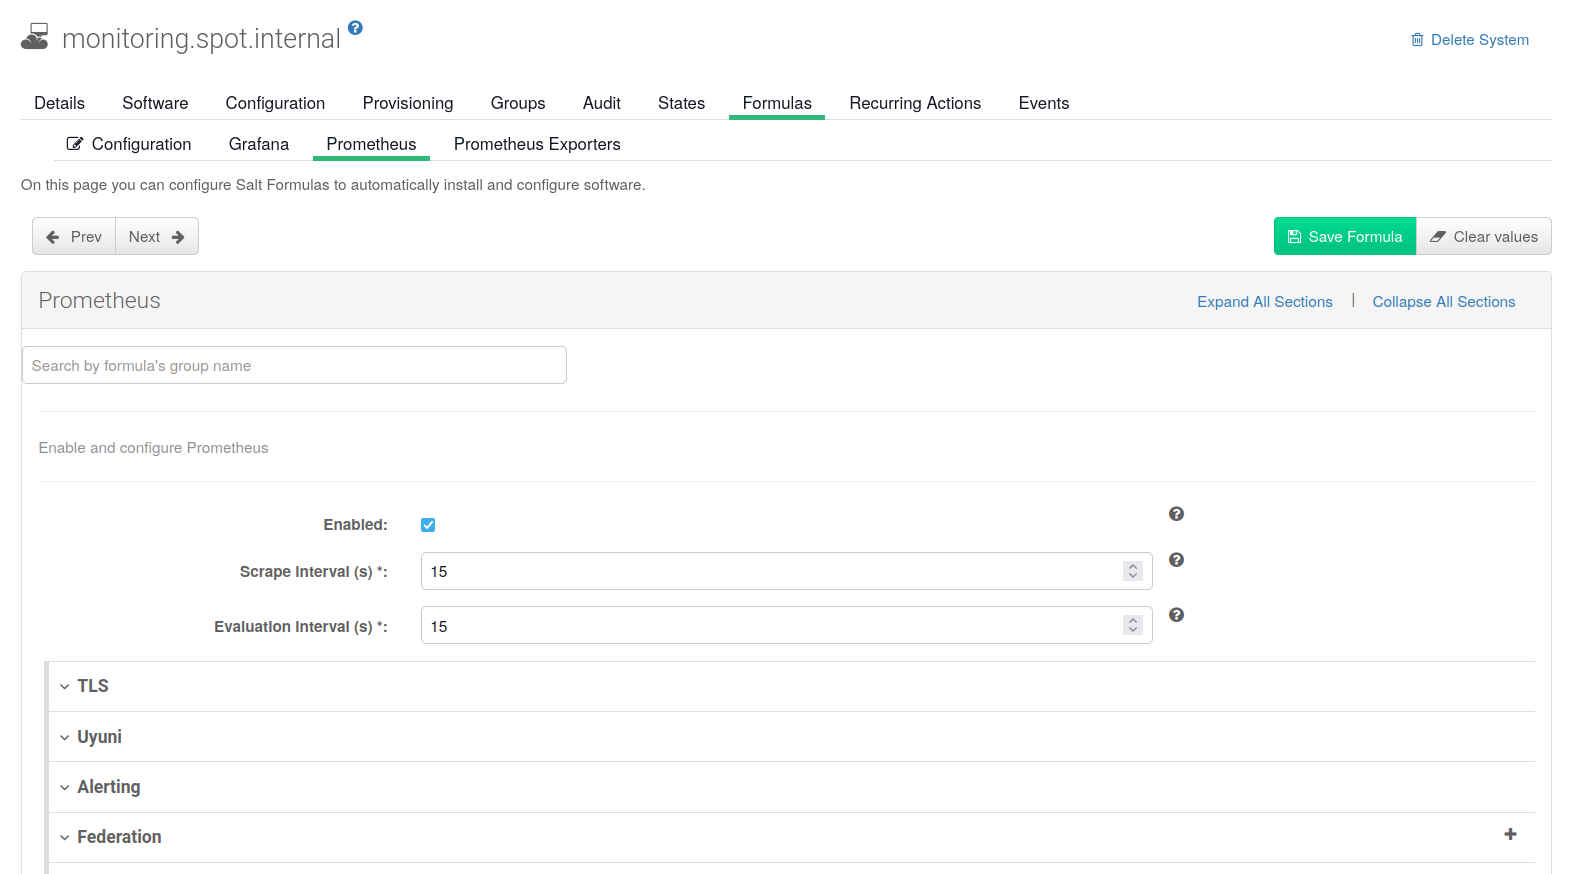
\includegraphics[width=15cm]{figures/prometheus-formula.png}
	\caption{Az Uyuni webes felületéről könnyen módosíthatjuk a Prometheus szerver alapvető beállításait.}
	\label{fig:prometheus-formula}
\end{figure}

\subsection{Konténerhoszt monitorozása}
A monitoring rendszer kialakítása során nehézséget jelentett, hogy openSUSE Leap Micro-ra nem volt hivatalosan elérhető a Node exporter szoftvercsomag formájában. Emiatt eleinte a konténerhoszt monitorozására nem volt lehetőségem. A megoldást az jelentette, hogy az exportert egy konténerben telepítettem a virtuális gépre. Mivel a konténer azonban a gazdagéptől elkülönülten fut, ezért módosítani kellett a konténer futtatásához használt parancsot. A \texttt{--path.rootfs=/host} kapcsoló beállításával az exporter már a konténerből is képes volt elérni a gazdagép metrikáit, így ezt a hosztot sikerült bevonni a monitoring rendszerbe.

\subsection{Tűzfal beállítása}
Az operációs rendszerek telepítése során a tűzfal engedélyezését választottam. Ez azt jelentette, hogy szinte minden port zárva volt a külvilág felé, így a Prometheus szerver sem tudta elérni az exporterek által szolgáltatott adatokat.

Ahhoz, hogy a monitoring rendszer az elvárt módon működjön, szükséges volt a tűzfalszabályok módosítása. A telepített rendszereken a \texttt{firewalld} az alapértelmezett tűzfal, melynek a beállításait a \texttt{firewall-cmd} segédprogram segítségével tudtam módosítani~(\ref{lst:firewalld-add-port}.~kódrészlet első~sora). A kódrészlet harmadik sorában a szükséges portok kinyitását követő állapot látható az Uyunit futtató szerver esetében, a monitoring rendszerben használt exportereket, rövid leírásukat és a kapcsolódó portszámokat \aref{tab:monitoring-exporters}.~táblázat tartalmazza.

\vspace{2mm}
\begin{lstlisting}[caption=Tűzfalszabályok módosítása.,label=lst:firewalld-add-port, numbers=left,escapechar=?]
	?\underline{uyuni:$\sim$ \#}? firewall-cmd --permanent --add-port=9117/tcp
	?\underline{uyuni:$\sim$ \#}? firewall-cmd --list-ports
	5556/tcp 5557/tcp 9100/tcp 9117/tcp 9187/tcp 9800/tcp
\end{lstlisting}

\begin{table}[h]
	\setlength{\tabcolsep}{5pt}
	\renewcommand{\arraystretch}{1.3}
	\centering
	\begin{tabular}{||l l m{7.6cm}||}
		\hline
		Portszám & Exporter & Leírás \\
		\hline\hline
		5556 & Tomcat JMX exporter & Az Uyuni működéséhez szükséges Tomcat alkalmazás Java-processzéről jelenít meg adatokat (pl.~szálak, memóriahasználat). \\
		\hline
		5557 & Taskomatic JMX exporter & Az Uyuni által használt Tascomatic alkalmazás Java-processzéről jelenít meg adatokat (pl.~szálak, memóriahasználat). \\
		\hline
		9090 & Prometheus exporter & A Prometheus állapotáról tesz közzé adatokat (pl.~hibás lekérések száma, lekérések mérete).  \\
		\hline
		9100 & Node exporter & Linux hosztokról publikál számos hardver- és kernelmetrikát (pl.~erőforráshasználat, kontextusváltások). \\
		\hline
		9117 & Apache exporter & Az Apache webszerverről ad meg mérőszámokat (pl.~egyes HTTP-státuszkódokhoz tartozó lekérdezések száma, \acrshort{cpu}-idő).  \\
		\hline
		9187 & PostgreSQL exporter & Az Uyuni által használt PostgreSQL adatbázismotorról oszt meg adatokat (pl.~zárak száma, rekordlekérdezési és frissítési ráta).  \\
		\hline
		9800 & Taskomatic exporter & Az Uyuni által használt Taskomatic feladatütemező metrikáit jeleníti meg (pl.~elvégzett feladatok száma, aktuális szálak száma).  \\
		\hline
	\end{tabular}
	\caption{A monitoring rendszerben használt Prometheus exporterek a hozzájuk tartozó portszámokkal.}
	\label{tab:monitoring-exporters}
\end{table}

% tikz ábra beszúrása
\begin{figure}[ht]
	\centering
	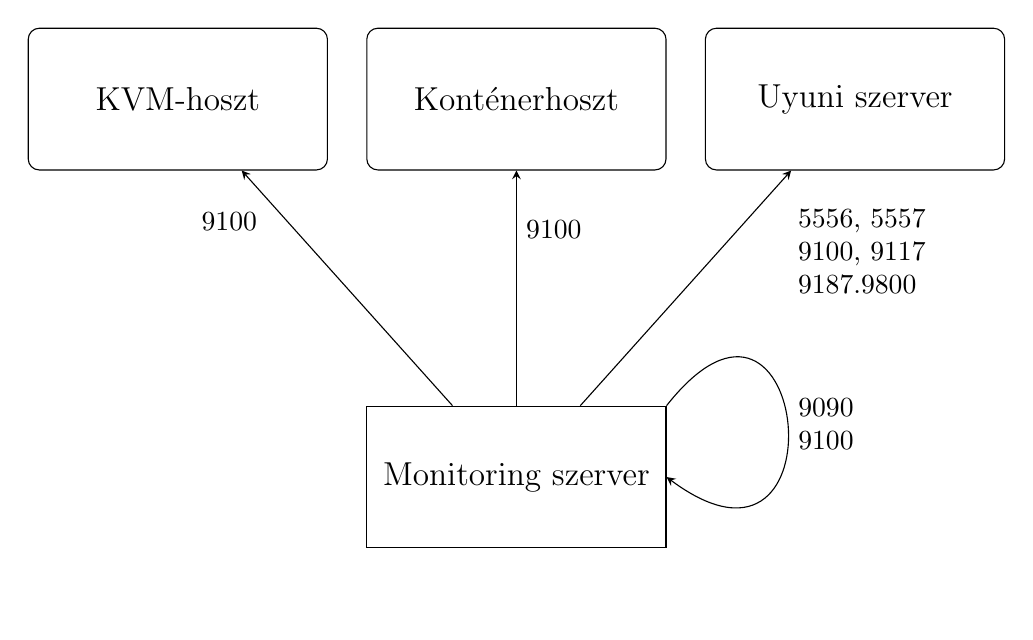
\begin{tikzpicture}[node distance=4.3cm]
	\tikzstyle{rect} = [rectangle, draw, minimum width=3.8cm, minimum height=1.8cm, text centered, font=\fontsize{12}{12}\selectfont]
	\tikzstyle{arrow} = [->,>=stealth]
	
	\node (kvm) [rect, rounded corners] {KVM-hoszt};
	\node (containers) [rect, rounded corners, right of = kvm] {Konténerhoszt};
	\node (uyuni) [rect, rounded corners, right of = containers] {Uyuni szerver};
	\node (monitoring) [rect, below of = containers, yshift=-0.5cm] {Monitoring szerver};
	
	\draw [arrow] (monitoring) to node[above left, near end, xshift=-10, yshift=-4, align=left] {9100} (kvm);
	\draw [arrow] (monitoring) to node[near end, right] {9100} (containers);
	\draw [arrow] (monitoring) to node[near end, right, align=left, xshift=18, yshift=-8] {5556, 5557\\9100, 9117\\9187.9800} (uyuni);
	\draw [arrow, loop, bend left] (monitoring.north east) to[out=150, in=60, looseness=8, align=left, xshift=3] node[right] {9090\\9100} (monitoring.east);
\end{tikzpicture}

	\caption{A monitoring rendszerbe bevont gépek a rajtuk futó exporterek által használt portokkal.}
	\label{fig:monitoring-setup}
\end{figure}